% implementierung.tex
%!TEX root = ../thesis.tex
\definecolor{lightblue}{RGB}{150,180,255}

\section{Verwendete Technologien}
\label{section:technologies}

In diesem Abschnitt wird knapp beschrieben, welche Technologien verwendet wurden und warum diese sinnvoll sind.

\subsection{R, RStudio, Pakete}

Die Programmiersprache R wurde ursprünglich für statistische Zwecke entwickelt. Die Hauptmerkmale sind eine mathematisch orientierte Syntax und implizites Typecasting. Dies in Kombination mit den über 8000 verfügbaren Paketen auf den CRAN-Servern\footnote{The Comprehensive R Archive Network: \url{https://cran.r-project.org/}} macht R zu einer universell einsetzbaren Sprache, perfekt geeignet für die Umsetzung einer Simulation der Kanalkodierung.\cite{rmanual}

\begin{figure}[t]
\centering
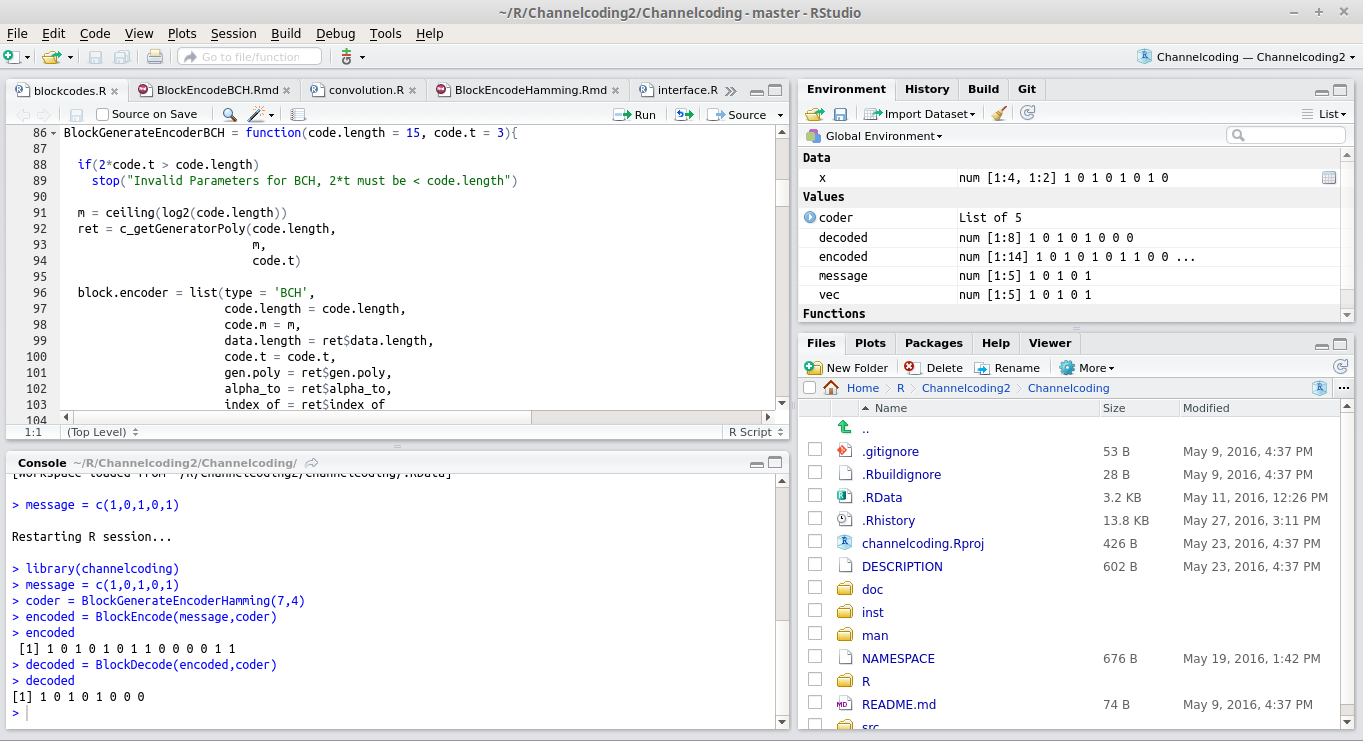
\includegraphics[width=\ScaleIfNeeded]{pictures/rstudio}
\caption{RStudio Screenshot}
\label{pic:rstudio}
\end{figure}

Als Entwicklungsumgebung wurde RStudio verwendet, in Abbildung~\ref{pic:rstudio} ist dessen Standardansicht abgebildet. Vor allem die einfache Installation von R-Paketen und die übersichtliche Darstellung von Daten machen RStudio zu einer angenehmen Entwicklungsumgebung. Zum entwickeln von R-Paketen ist es außerdem noch sinnvoll die Pakete \emph{devtools} und \emph{roxygen2} zu installieren. \emph{Devtools} bietet einige sehr hilfreiche Funktionen zum Erstellen und Kompilieren eines R-Pakets.\cite{devtools} Ähnlich wie \emph{JavaDoc} ermöglicht \emph{roxygen2} die verwendung von Annotations im Code, welche einerseits die Dokumentation für das Paket erzeugen, andererseits aber auch durch \emph{@examples} Tests definieren und mittels \emph{@export} bestimmt wird, welche Funktionen der Nutzer später zur Verfügung hat und welche nur intern sind.(vgl. \emph{private} und \emph{public})\cite{roxygen}

\subsection{C, C++, Rcpp}

Wie in \cite{Rextension} beschrieben sollten beim Implementieren eines R-Pakets stets die Schwächen von R berücksichtigt werden. Diese sind im Wesentlichen die schwache Typisierung und die schlechte Performance bei iterativen Berechnungen. Deswegen sollten rechenintensive Codeabschnitte in einer performanteren Programmiersprache wie etwa C oder C++ implementiert werden. Für deren Integration bietet R zwei Schnittstellen:

\begin{itemize}
\item Das \emph{.C() Interface}
\item Das \emph{.Call() Interface}
\end{itemize}

Ersteres ist die einfachste Möglichkeit C Code in R auszuführen, es werden keine speziellen Datentypen verwendet. Dadurch müssen die Variablen allerdings kopiert werden und es steht im C Code keinerlei Wissen über R zur Verfügung.
Mit \emph{.Call()} wurden eigene C++ Klassen, die R Datentypen repräsentieren, eingeführt. Dadurch müssen die Variablen nicht mehr kopiert werden und es kann im C/C++ Code vom Wissen über die R Datentypen profitiert werden.\cite{wickham2015r} Allerdings muss der Entwickler sich erst in die etwas verwirrende Verwendung der Schnittstelle einarbeiten. Abhilfe schafft hier das \emph{Rcpp}-Paket, welches die Integration von C/C++ in R extrem einfach macht. Es werden automatisch Wrapper für die \emph{.Call()} Schnittstelle generiert und es stehen viele hilfreiche Funktionen zur Verfügung. Auch das Kompilieren übernimmt \emph{Rcpp}. Eine ausführliche Beschreibung des Pakets findet sich in \cite{wickham2015advanced}.

\subsection{R Markdown und \LaTeX}

Für die Visualisierung der Kanalkodierung bietet RStudio in Kombination mit dem Paket \emph{RMarkdown} eine hervorragende Möglichkeit. Grundsätzlich wird in .Rmd Dateien \LaTeX~Code  mit R~Code verwendet, wodurch dynamisch Dokumente erzeugt werden können. In Abbildung~\ref{pic:RMarkdown} ist der Ablauf abgebildet. \emph{Knitr} führt zunächst den R Code aus, die entstandene .md Datei wird anschließend mit dem in RStudio integrierten Programm \emph{Pandoc} zum gewünschten Output, in diesem Fall PDF, gerendert.\cite{rmarkdown}

\begin{figure}[ht]
\centering

\includegraphics[width=\ScaleIfNeeded]{pictures/RMarkdown}
\caption{RMarkdown Schema, Quelle: \cite{rmarkdown}}
\label{pic:RMarkdown}
\end{figure}




\section{R-Paket Schnittstelle}
\label{section:interface}

In diesem Abschnitt werden alle Funktionen, die dem Nutzer im R-Paket zur Verfügung stehen, beschrieben.

\subsection{Kodierung}

\label{sec:interface_genHamming}
% BlockGenerateEncoderHamming
\begin{longtable}{|p{\textwidth}|}
\hline
\rowcolor{lightblue}
BlockGenerateEncoderHamming
\\
\hline
\\
\texttt{BlockGenerateEncoderHamming(code.length, data.length)}\\
\\
Erzeugt einen Blockkodierer für Hamming-Kodes.\\
\\
\textbf{Argumente:}\\
\texttt{code.length} - Länge der Kodewörter.\\
\texttt{data.length} - Länge der Datenwörter.\\
\\
\textbf{Rückgabewert:}\\
Hamming-Kode, abgebildet als Liste mit folgenden Feldern:
\vspace{4mm}
\begin{itemize}
\renewcommand\labelitemi{--}
\itemsep-.5em % spacing between items
\item code.length
\item data.length
\item gen.matrix
\item check.matrix
\end{itemize}
\\
\hline
\caption{BlockGenerateEncoderHamming}
\end{longtable}

\label{sec:interface_genBCH}
% BlockGenerateEncoderBCH
\begin{longtable}{|p{\textwidth}|}
\hline
\rowcolor{lightblue}
BlockGenerateEncoderBCH
\\
\hline
\\
\texttt{BlockGenerateEncoderBCH(code.length, code.t)}\\
\\
Erzeugt einen Blockkodierer für BCH-Kodes.\\
\\
\textbf{Argumente:}\\
\texttt{code.length} - Länge der Kodewörter.\\
\texttt{code.t} - Anzahl der verbesserbaren Fehler pro Kodewort.\\
\\
\textbf{Rückgabewert:}\\
BCH-Kode, abgebildet als Liste mit folgenden Feldern:
\vspace{4mm}
\begin{itemize}
\renewcommand\labelitemi{--}
\itemsep-.5em % spacing between items
\item code.length
\item data.length
\item gen.matrix
\item check.matrix
\end{itemize}
\\
\hline
\caption{BlockGenerateEncoderHamming}
\end{longtable}

\clearpage
\label{sec:interface_encode}
\begin{longtable}{|p{\textwidth}|}
\hline
\rowcolor{lightblue}BlockEncode\\
\hline
\\
\texttt{BlockEncode(message, block.encoder, visualize)}\\
\\
Kodiert die Nachricht mithilfe des in block.encoder angegebenen Blockkodes. Die zu kodierende Nachricht wird dazu in Blöcke der Datenwortlänge des Kodierers aufgeteilt und ggf. 0en angehängt um alle Blöcke gleich lang zu machen. \\
\\
\textbf{Argumente:}\\
\texttt{message} - Nachricht die kodiert wird, als binärer Vektor.\\
\texttt{block.encoder} - Blockkodierer der mit den Funktionen \emph{BlockGenerateEncoderHamming, BlockGenerateEncoderBCH} erzeugt werden kann. Standard: \emph{BlockGenerateEncoderBCH(15,3)}\\
\texttt{visualize} - Wenn TRUE wird ein Visualisierungs-PDF erstellt. Standard: FALSE\\
\\
\textbf{Rückgabewert:}\\
Die kodierte Nachricht als binärer Vektor.\\
\\
\hline
\caption{BlockEncode}
\end{longtable}

\subsection{Dekodierung}

\label{sec:interface_decode}
\begin{longtable}{|p{\textwidth}|}
\hline
\rowcolor{lightblue}BlockDecode\\
\hline
\\
\texttt{BlockDecode(code, block.encoder, visualize)}\\
\\
Dekodiert die Nachricht mithilfe des in block.encoder angegebenen Blockkodes. Die zu dekodierende Nachricht wird dazu in Blöcke der Kodewortlänge des Kodierers aufgeteilt und ggf. 0en angehängt um alle Blöcke gleich lang zu machen. \\
\\
\textbf{Argumente:}\\
\texttt{me} - Nachricht die kodiert wird, als binärer Vektor.\\
\texttt{block.encoder} - Blockkodierer der mit den Funktionen \emph{BlockGenerateEncoderHamming, BlockGenerateEncoderBCH} erzeugt werden kann. Standard: \emph{BlockGenerateEncoderBCH(15,3)}\\
\texttt{visualize} - Wenn TRUE wird ein Visualisierungs-PDF erstellt. Standard: FALSE\\
\\
\textbf{Rückgabewert:}\\
Die kodierte Nachricht als binärer Vektor.\\
\\
\hline
\caption{BlockEncode - Funktionserklärung}
\end{longtable}

\label{sec:interface_simulation}
\begin{longtable}{|p{\textwidth}|}
\hline
\rowcolor{lightblue}BlockSimulation\\
\hline
\\
\texttt{BlockSimulation(coder, msg.length, min.db, max.db, db.interval, iterations.per.db, punctuation.matrix, visualize)}\\
\\
Automatische Simulation eines Kodierungs- und Dekodierungsverfahrens von Blockkodes. Nach dem Kodieren wird der resultierende Kode verrauscht(siehe Funktion~\ref{func:applynoise}) und im Anschluss dekodiert. Für das jeweilige Signal-Rausch-Verhältnis(SNR) wird dieses Verfahren mehrmals (iterations.per.db) wiederholt und am Ende der Durchschnitt der Bitfehlerrate berechnet.\\
\\
\textbf{Argumente:}\\
\texttt{coder} - Blockkodierer der mit den Funktionen \emph{BlockGenerateEncoderHamming, BlockGenerateEncoderBCH} erzeugt werden kann. Standard: \emph{BlockGenerateEncoderBCH(15,3)}\\
\texttt{decode.iterations} - Anzahl von Iterationen bei der Dekodierung. Standard: 5\\
\texttt{msg.length} - Länge der Nachricht. Standard: 100\\
\texttt{min.db} - Untergrenze des SNR. Standard: 0.1\\
\texttt{max.db} - Obergrenze des SNR. Standard: 2.0\\
\texttt{db.interval} - Schrittweite pro Erhöhung des SNR. Standard: 0.1\\
\texttt{iterations.per.db} - Iterationen pro SNR zur Durchschnittsbildung. Standard: 100\\
\texttt{visualize} - Wenn TRUE wird PDF-Bericht erstellt. Standard: FALSE\\
\\
\textbf{Rückgabewert:}\\
Dataframe mit einer Bitfehlerrate für jedes SNR.\\
\\
\hline
\caption{BlockSimulation}
\label{func:block_simu}
\end{longtable}



\subsection{Gemeinsame Funktionen}
\label{sec:interface_applynoise}
\begin{longtable}{|p{\textwidth}|}
\hline
\rowcolor{lightblue}
ApplyNoise\\
\hline
\\
\texttt{ApplyNoise(msg, SNR.db, binary)}\\
\\
Verrauscht ein Signal basierend auf das AWGN (additive white gaussian noise) Modell. Das ist das Standardmodell für die Simulation eines Übertragungskanals.\\
\\
\textbf{Argumente:}\\
\texttt{msg} - Nachricht die verrauscht wird.\\
\texttt{SNR.db} - Signal/Rausch-Verhältnis des Übertragungskanals. Standard: 3.0\\
\texttt{binary} - Blockkode-Parameter. Nicht zu verwenden! Standard: FALSE\\
\\
\textbf{Rückgabewert:}\\
Verrauschtes Signal.\\
\\
\hline
\caption{ApplyNoise - Funktionserklärung}
\label{func:applynoise}
\end{longtable}

\label{sec:interface_channelsimulation}
% ChannelcodingSimulation.tex
\begin{longtable}{|p{\textwidth}|}
\hline
\rowcolor{lightblue}ChannelcodingSimulation\\
\hline
\\
\texttt{ChannelcodingSimulation(msg.length, min.db, max.db, db.interval, iterations.per.db, turbo.decode.iterations, visualize)}\\
\\
Simulation of channelcoding techniques (blockcodes, convolutional codes and turbo codes) and comparison of their bit-error-rates.\\
\\
\textbf{Arguments:}\\
\texttt{msg.length} - Message length of the randomly created messages to be encoded. Default: 100\\
\texttt{min.db} - Minimum SNR to be tested. Default: 0.1\\
\texttt{max.db} - Maximum SNR to be tested. Default: 2.0\\
\texttt{db.interval} - Step between two SNRs tested. Default: 0.1\\
\texttt{iterations.per.db} - Number of encode and decode processes per SNR. Default: 100\\
\texttt{turbo.decode.iterations} - Number of decoding iterations inside the turbo decoder. Default: 5\\
\texttt{visualize} - If true a PDF report is generated. Default: FALSE\\
\\
\textbf{Returns:}\\
Distorted message containing noise.\\
\\
\hline
\end{longtable}

\label{sec:interface_plotdata}
% PlotSimulationData.tex
\begin{longtable}{|p{\textwidth}|}
\hline
\rowcolor{lightblue}PlotSimulationData\\
\hline
\\
\texttt{PlotSimulationData(\dots)}\\
\\
Stellt mehrere mitgegebene Dataframes in einem Diagramm dar. Damit kann man verschiedene Kanalkodierungsverfahren miteinander vergleichen.\\
\\
\textbf{Argumente:}\\
\texttt{\dots} - Dataframes die mit den Simulationsfunktionen erzeugt wurden.\\	
\\
\hline
\caption[PlotSimulationData]{PlotSimulationData - Funktionserklärung}
\end{longtable}



\section{Blockkodes}
\label{section:impl_block}
In diesem Abschnitt wird beschrieben, wie die Theorie aus Kapitel~\ref{chapter:theory} im R-Paket umgesetzt wurde.

\subsection{Hamming}

\begin{lstlisting}[caption=Erzeugung der Generator- und Kontrollmatrix, label={lst:genHamming}, float=ht]
r = code.length - data.length
p = 1:code.length
p = p[(log2(p)%%1)!=0 ]
p = sapply(p, function(x) binVector(x,r))
p = matrix(p, nrow = r)

check.matrix = cbind(p,diag(r))
gen.matrix = cbind(diag(data.length),t(p))
\end{lstlisting}

\begin{lstlisting}[caption=Dekodierung eines Hamming-Kodes, label={lst:decHamming}, float=ht]
result = as.vector((block.encoder$check.matrix %*% message) %% 2)

FindErrors = function(){
    i = 1
    function(x){
      if(isTRUE(identical(result,x))){
      	message[i] <<- (message[i]+1)%%2
      }
      i <<- i+1
      x
    }
}

apply(block.encoder$check.matrix, 2, FindErrors())

\end{lstlisting}

Die Erzeugung eines Hammingkodierers erfolgt mit dem R-Code in Listing~\ref{lst:genHamming}, der Ablauf entspricht dem in Kapitel~\ref{section:hamming}. Zunächst werden die Zahlen 1 bis \emph{code.length} als binäre Vektoren in \emph{p} spaltenweise geschrieben, danach die 2er Potenzen wieder entfernt. Die \emph{check.matrix} ist dann $(p \mid I_r)$, die \emph{gen.matrix} entspricht $(p \mid I_{data.length})$.
\newblock
Die Kodierung ist lediglich eine Matrixmultiplikation des Datenwortes mit der Generatormatrix des Hamming-Kodes. Für die Dekodierung wird der R-Code in \ref{lst:decHamming} verwendet. Das Kodewort wird mit der Kontrollmatrix multipliziert und das Ergebnis in \emph{result} gespeichert. Die Hilfsfunktion \emph{FindErrors()} sucht nun nach dem Vektor \emph{result} in den Spalten der Kontrollmatrix, bei einem Treffer wird die entsprechende Stelle im Kodewort korrigiert.



\subsection{BCH}

Im Gegensatz zu der Implementierung der Hamming-Kodes, welche sich gut in R umsetzen ließen, sind die BCH-Kodes in C umgesetzt. Als Basis dient der von Robert Morelos-Zaragoza, dem Autor von \cite{morelos2006art}, bereitgestellte Code. Dieser ist auf der ECC-Page~\cite{eccpage} verfügbar und implementiert die in Kapitel~\ref{sec:bch} beschriebenen Schritte. Um ein Generatorpolynom zu erzeugen, muss zunächst wie in Tabelle~\ref{table:gf} $GF(2^m)$ in Index- und Polynomdarstellung konstruiert werden. Dies geschieht in Listing~\ref{lst:bch_alpha}. In \emph{alpha\_to} sind die Polynome als Integer, welche die binäre Vektordarstellung repräsentieren, gespeichert. In \emph{index\_of} stehen die Indizes der Elemente, es gilt: \texttt{index\_of[alpha\_to[i]] = i}.
\vspace{0.5cm}
\begin{lstlisting}[caption=Konstruieren des $GF(2^m)$, label={lst:bch_alpha}, language=C]
  mask = 1;
  alpha_to[m] = 0;
  for (i = 0; i < m; i++) {
    alpha_to[i] = mask;
    index_of[alpha_to[i]] = i;
    if (p[i] != 0)		/* p = primitives Polynom */
      alpha_to[m] ^= mask;
    mask <<= 1;
  }
  index_of[alpha_to[m]] = m;
  mask >>= 1;
  for (i = m + 1; i < n; i++) {	// n = 2^m -1
    if (alpha_to[i - 1] >= mask)
      alpha_to[i] = alpha_to[m] ^ ((alpha_to[i - 1] ^ mask) << 1);
    else
      alpha_to[i] = alpha_to[i - 1] << 1;
    index_of[alpha_to[i]] = i;
  }
  index_of[0] = -1;
\end{lstlisting}
\clearpage
\begin{lstlisting}[caption=Finden aller Zykel $\mod 2^m-1$, label={lst:bch_cycle}, language=C++]
  do {
    ii = 0;
    do {
      ii++;
      cycle[jj][ii] = (cycle[jj][ii - 1] * 2) % n;
      size[jj]++;
      aux = (cycle[jj][ii] * 2) % n;
    } while (aux != cycle[jj][0]);
    ll = 0;
    do {
      ll++;
      test = 0;
      for (ii = 1; ((ii <= jj) && (!test)); ii++)
        for (kaux = 0; ((kaux < size[ii]) && (!test)); kaux++)
          if (ll == cycle[ii][kaux])
            test = 1;
    } while ((test) && (ll < (n - 1)));
    if (!(test)) {
      jj++; /* next cycle set index */
        cycle[jj][0] = ll;
        size[jj] = 1;
    }
  } while (ll < (n - 1));
\end{lstlisting}

\begin{lstlisting}[caption=Suchen der Nullstellen in den Zykeln, label={lst:bch_roots}, language=C++]
d = 2 * t + 1;
kaux = 0;
rdncy = 0;
for (ii = 1; ii <= nocycles; ii++) {
    min[kaux] = 0;
    test = 0;
    for (jj = 0; ((jj < size[ii]) && (!test)); jj++)
    for (root = 1; ((root < d) && (!test)); root++)
    if (root == cycle[ii][jj]) {
        test = 1;
        min[kaux] = ii;
    }
    if (min[kaux]) {
        rdncy += size[min[kaux]];
        kaux++;
    }
}
noterms = kaux;
kaux = 1;
for (ii = 0; ii < noterms; ii++)
for (jj = 0; jj < size[min[ii]]; jj++) {
    zeros[kaux] = cycle[min[ii]][jj];
    kaux++;
}
\end{lstlisting}

\begin{lstlisting}[caption=Konstruieren des Generatorpolynoms, label={lst:bch_genpoly}, language=C++]
g[0] = alpha_to[zeros[1]];
g[1] = 1;
for (ii = 2; ii <= rdncy; ii++) {	//rdncy = n - k
    g[ii] = 1;
    for (jj = ii - 1; jj > 0; jj--)
    if (g[jj] != 0)
    g[jj] = g[jj - 1] ^ alpha_to[(index_of[g[jj]] + zeros[ii]) % n];
    else
    g[jj] = g[jj - 1];
    g[0] = alpha_to[(index_of[g[0]] + zeros[ii]) % n];
}
\end{lstlisting}



Als nächstes werden in Listing~\ref{lst:bch_cycle} alle Zykel für $x \mod 2^m-1$ erzeugt. Danach werden in Listing~\ref{lst:bch_roots} die relevanten Nullstellen $\alpha^{1,...,2t}$ in den Zykeln lokalisiert. Schließlich wird in Listing~\ref{lst:bch_genpoly} analog zu den Definitionen \ref{def:minimal} und \ref{def:genpoly} das Generatorpolynom konstruiert. Die Kodierung, wie beschrieben in Definition~\ref{def:encode}, erfolgt in Listing~\ref{lst:bch_encode}.
\vspace{0.5cm}
\begin{lstlisting}[caption=Kodierung mit dem Generatorpolynom, label={lst:bch_encode}, language=C++]
for (i = 0; i < length - k; i++)
	bb[i] = 0;
for (i = k - 1; i >= 0; i--) {
    feedback = input[i] ^ bb[length - k - 1];
    if (feedback != 0) {
        for (j = length - k - 1; j > 0; j--)
        	if (genPoly[j] != 0)
       			 bb[j] = bb[j - 1] ^ feedback;
        	else
       			 bb[j] = bb[j - 1];
        bb[0] = genPoly[0] && feedback;
        } else {
        	for (j = length - k - 1; j > 0; j--)
       			bb[j] = bb[j - 1];
        	bb[0] = 0;
    }
}
for (i = 0; i < length - k; i++)
	code[i] = bb[i];
for (i = 0; i < k; i++)
	code[i + length - k] = input[i];
return code;
\end{lstlisting}

Die Dekodierung der BCH-Kodes erfolgt exakt wie in Kapitel~\ref{sec:bch} beschrieben. An dieser Stelle wird jedoch auf Listings und eine detaillierte Beschreibung verzichtet, da vor allem die Implementierung des Berlekamp-Massey-Algorithmus sehr viele Schleifen und unübersichtlichen Code beinhaltet. Wer sich damit im Detail beschäftigen möchte sollte sich mit den Grundlagen in \cite[S. 54ff]{morelos2006art} und den Implementierungen auf der ECC-Page\cite{eccpage} auseinandersetzen.


